\documentclass[conference]{IEEEtran}
\IEEEoverridecommandlockouts

\usepackage[T1]{fontenc}
\usepackage{newtxtext,newtxmath}
\usepackage{cite}
\usepackage{amsmath}
\usepackage{graphicx}
\usepackage{booktabs}
\usepackage{url}
\usepackage[hidelinks]{hyperref}

\begin{document}

\title{AgroTech AI: Hybrid CNN--LLM Plant Disease Diagnosis and Context-Aware Advisory for Farmers}

\author{
\IEEEauthorblockN{Samresh Chaudhari}
\IEEEauthorblockA{\textit{Dept. of Information Technology} \\
\textit{VESIT, Mumbai, India}}
\and
\IEEEauthorblockN{Shrijeet Deshmukh}
\IEEEauthorblockA{\textit{Dept. of Information Technology} \\
\textit{VESIT, Mumbai, India}}
\and
\IEEEauthorblockN{Harsh Totani}
\IEEEauthorblockA{\textit{Dept. of Information Technology} \\
\textit{VESIT, Mumbai, India}}
\and
\IEEEauthorblockN{Chinmay Bhutada}
\IEEEauthorblockA{\textit{Dept. of Information Technology} \\
\textit{VESIT, Mumbai, India}}
\and
\IEEEauthorblockN{Prof. Archana Kshirsagar}
\IEEEauthorblockA{\textit{Dept. of Information Technology} \\
\textit{VESIT, Mumbai, India}}
}

\maketitle

\begin{abstract}
Disease classifiers used in farm advisory tools recognise only the crops they were trained on, while general chatbots know nothing about the farmer. We present AgroTech AI, an advisory platform built around a hybrid plant-disease diagnosis. A transfer-learned EfficientNetV2-B0 convolutional neural network (CNN), restricted to the classes of the plant the farmer names, and the Gemini multimodal large language model (LLM) diagnose a leaf photo independently and are combined by a weighted vote; plants outside the CNN's nine crops are diagnosed by Gemini, and the CNN works offline when Gemini is unavailable. An assistant grounds its answers in the farmer's profile, crops and earlier results. Trained on laboratory and field images, the CNN reaches 94.66\% accuracy on laboratory test images and 48.43\% on field photographs, compared with 12.41\% for a VGG16 baseline. A feature study on 28,242 yield records shows that adding crop type, country and year raises $R^2$ from $-0.20$ to 0.955.
\end{abstract}

\begin{IEEEkeywords}
plant disease detection, CNN, large language model, transfer learning, crop yield prediction, precision agriculture
\end{IEEEkeywords}

\section{Introduction}
Most farms in developing economies are small and have little access to agronomic expertise, so crop diseases and poor input choices reduce yields every season. Machine learning can help~\cite{kamilaris2018,liakos2018}, but current tools have three weaknesses. Image classifiers are accurate on curated datasets such as PlantVillage~\cite{hughes2015} but recognise only their training classes and degrade on field photographs~\cite{mohanty2016,singh2020plantdoc}. Multimodal LLMs~\cite{gemini2023} can describe almost any plant problem but need connectivity and can be confidently wrong. Most tools are also stateless and ignore the farmer's crops and history.

This paper makes three contributions:
\begin{itemize}
\item A hybrid diagnosis that restricts a CNN to the stated plant, maps an independent LLM diagnosis onto the CNN's labels and combines the two by a weighted vote, with an offline fallback.
\item A laboratory-versus-field evaluation showing that training on field photographs raises field accuracy from 12.41\% to 48.43\%.
\item A context-aware assistant that personalises advice from the farmer's own records.
\end{itemize}

\section{Related Work}
Mohanty et al.~\cite{mohanty2016} reached 99.35\% accuracy on 38 PlantVillage classes, but accuracy dropped on images from other sources. Ferentinos~\cite{ferentinos2018} extended this to 58 classes with VGG networks~\cite{simonyan2015}, and Singh et al.~\cite{singh2020plantdoc} showed with the PlantDoc field dataset that laboratory-trained models transfer poorly. For yield, van Klompenburg et al.~\cite{vanklompenburg2020} found weather and soil features and Random Forests~\cite{breiman2001} to be most common. Retrieval-augmented generation~\cite{lewis2020} grounds an LLM in external data, and ensemble theory~\cite{dietterich2000} shows that combining independent predictors reduces error. Table~\ref{tab:related} summarises the gap our system addresses.

\begin{table}[t]
\caption{Related Work}
\label{tab:related}
\centering
\footnotesize
\begin{tabular}{@{}p{0.13\columnwidth}p{0.38\columnwidth}p{0.38\columnwidth}@{}}
\toprule
\textbf{Work} & \textbf{Approach} & \textbf{Limitation} \\
\midrule
\cite{mohanty2016} & CNN, 38 PlantVillage classes & Closed set; lab images only \\
\cite{ferentinos2018} & VGG CNNs, 58 classes & Closed set \\
\cite{singh2020plantdoc} & CNNs on field images & Small dataset; closed set \\
\cite{gemini2023} & Multimodal LLM & Needs connectivity; not domain-tuned \\
Ours & Hybrid CNN + LLM with assistant & Field accuracy below lab accuracy \\
\bottomrule
\end{tabular}
\end{table}

\section{System Overview}
AgroTech AI is a web application with a React frontend, a Flask REST API and an SQLite database (Fig.~\ref{fig:arch}). Besides disease diagnosis and the assistant, it offers crop recommendation, soil analysis, fertilizer plans, yield estimates and a weather dashboard with field alerts. Every result is saved to the farmer's activity history, which the assistant uses as context.

\begin{figure}[t]
\centering
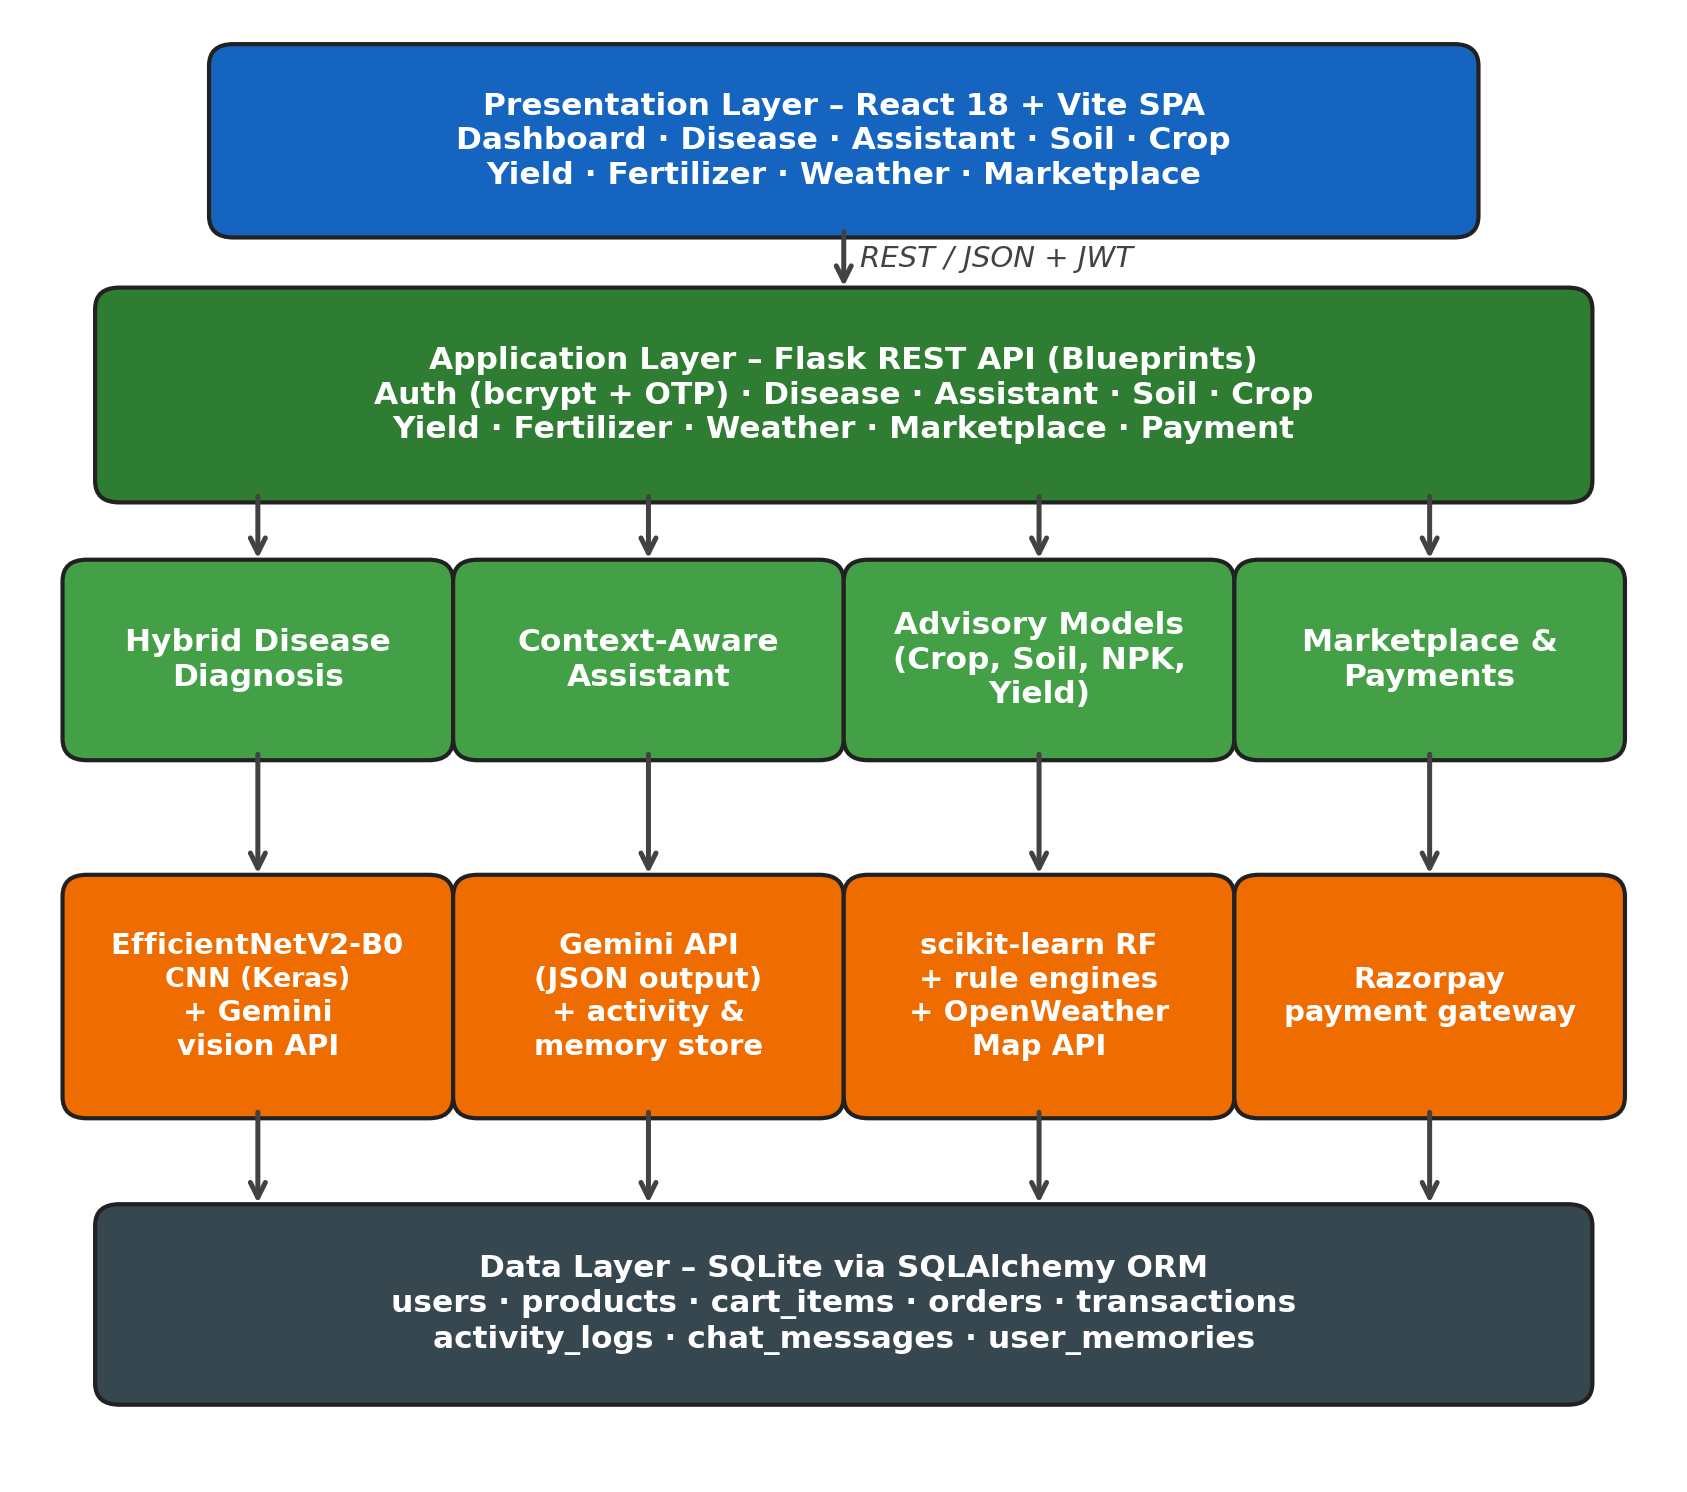
\includegraphics[width=\columnwidth]{figures/architecture.png}
\caption{System architecture.}
\label{fig:arch}
\end{figure}

\section{Method}

\subsection{Plant-Conditioned CNN}
The CNN outputs probabilities $p(c)$ over 33 classes. Since the farmer names the plant $k$, classes of other plants are removed. With $\pi(c)$ the plant of class $c$:
\begin{equation}
p_C(c \mid k) = \frac{p(c)\,\mathbf{1}[\pi(c) = k]}{\sum_{c'} p(c')\,\mathbf{1}[\pi(c') = k]}
\label{eq:mask}
\end{equation}

\subsection{LLM Diagnosis and Fusion}
Gemini receives the image and the plant name and returns a structured diagnosis. For plants the CNN covers, it also maps its answer onto one of the CNN's classes $m$ with confidence $g$, without seeing the CNN's prediction. For a plant with $n$ classes:
\begin{equation}
p_G(c) = \begin{cases} g & \text{if } c = m \\ \dfrac{1 - g}{n - 1} & \text{otherwise} \end{cases}
\label{eq:gemini}
\end{equation}
\begin{equation}
S(c) = 0.6\, p_G(c) + 0.4\, p_C(c \mid k), \qquad \hat{c} = \arg\max_{c} S(c)
\label{eq:fusion}
\end{equation}
The result is labelled \textit{agree}, \textit{gemini\_preferred} or \textit{cnn\_preferred} according to which model wins, and \textit{gemini\_only} when Gemini finds a condition outside the CNN's classes. Gemini is weighted higher because the CNN is weaker on field photographs. If Gemini is unavailable, the CNN result is returned with the reason (Fig.~\ref{fig:pipeline}).

\begin{figure}[t]
\centering
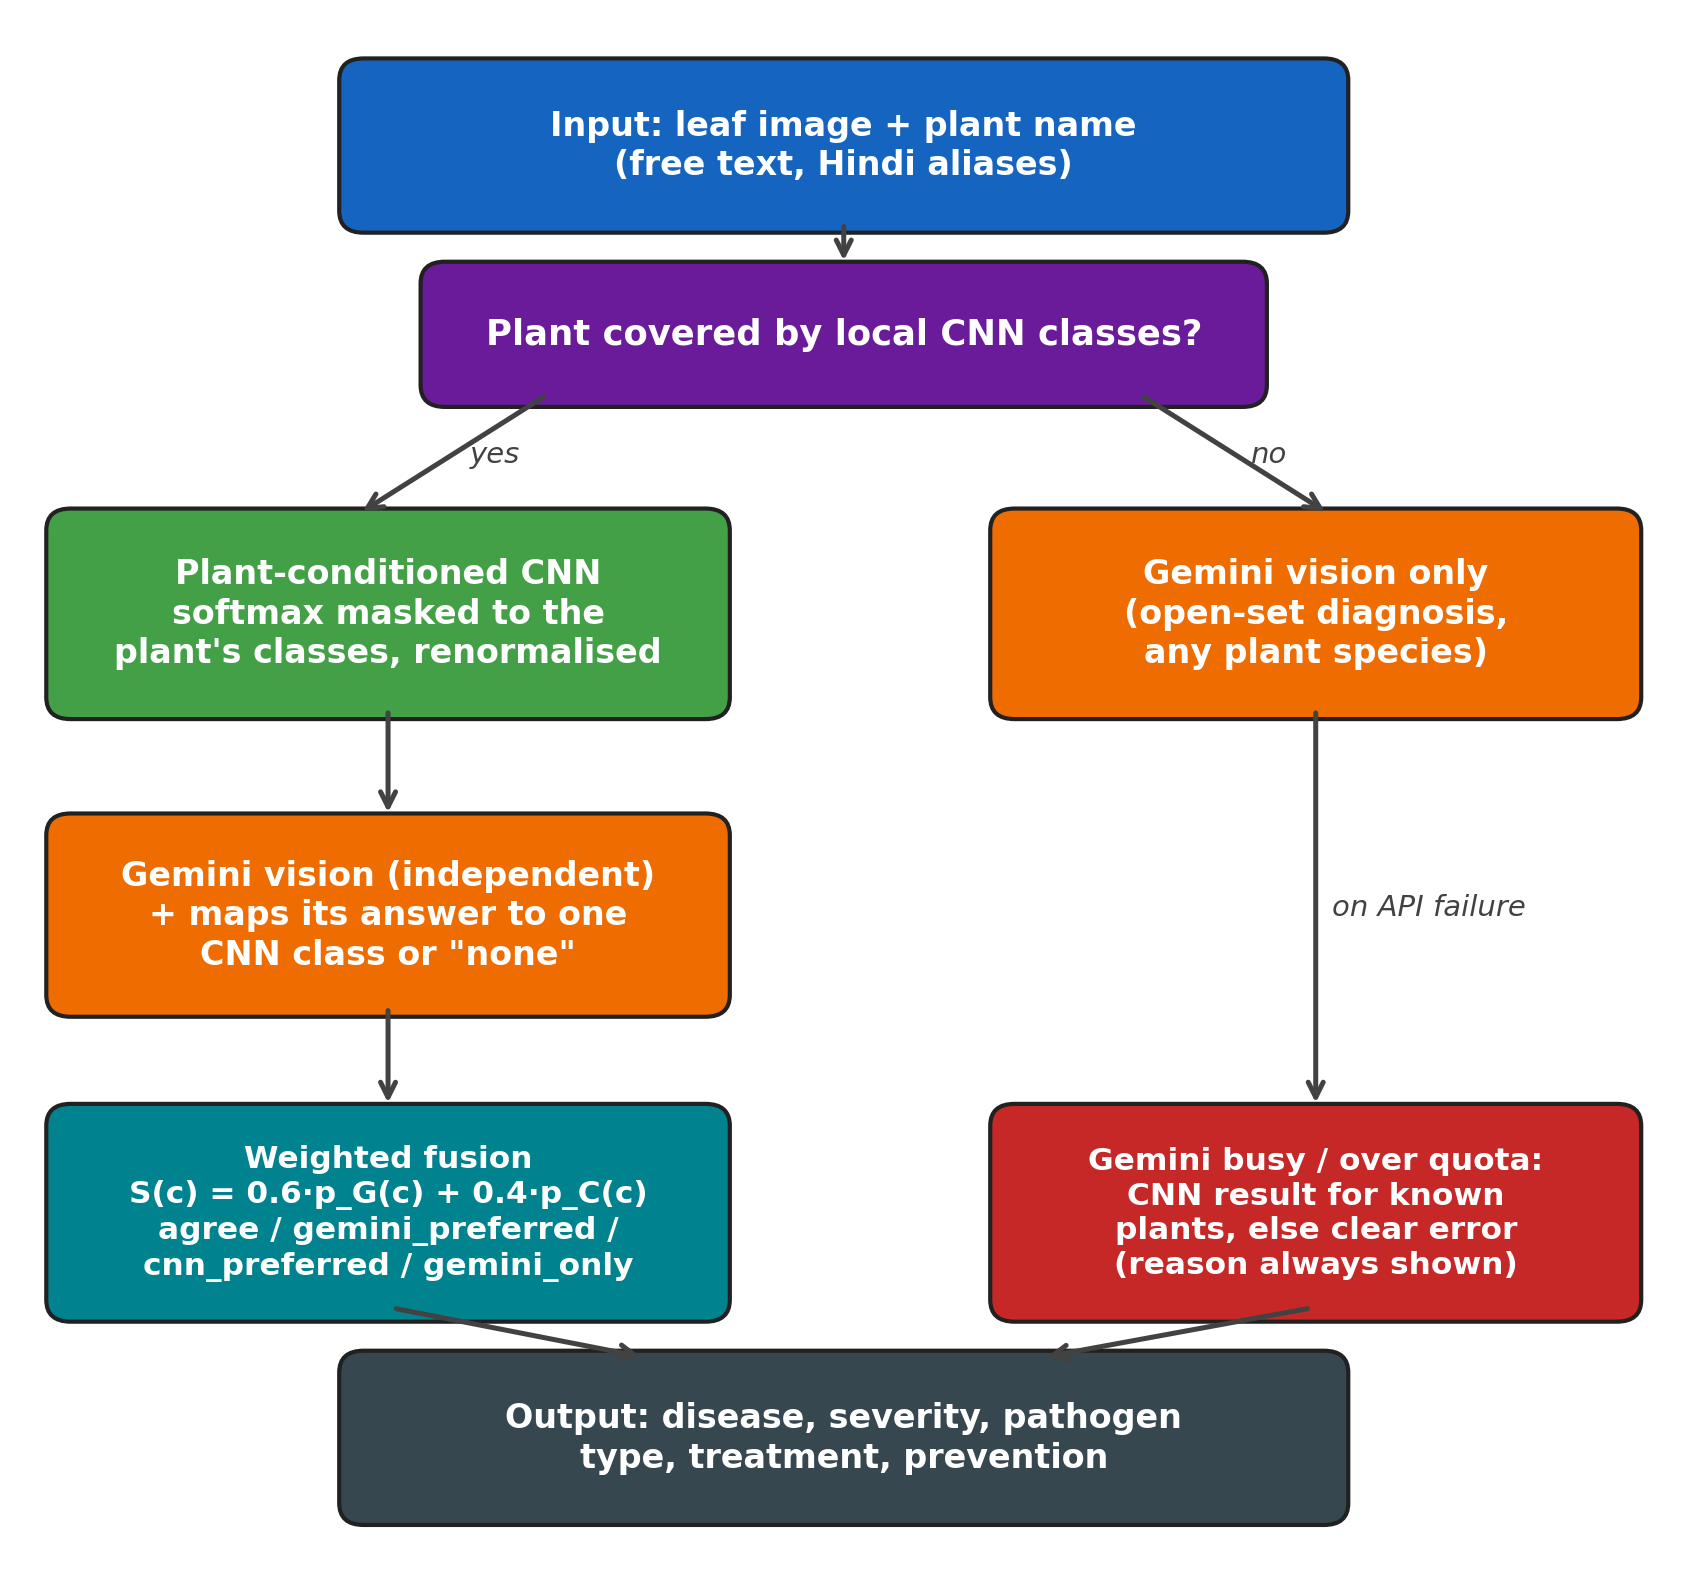
\includegraphics[width=0.9\columnwidth]{figures/pipeline.png}
\caption{Hybrid diagnosis pipeline.}
\label{fig:pipeline}
\end{figure}

\subsection{Context-Aware Assistant}
For each message the assistant builds a prompt from the farmer's profile, recorded crops, up to 40 remembered facts, the 15 latest results and the last 20 chat turns. New facts stated by the farmer are stored, and the farmer can view or delete them.

\section{Experimental Setup}
\textbf{Data.} We merged PlantVillage~\cite{hughes2015} laboratory images and PlantDoc~\cite{singh2020plantdoc} field photographs into 22,686 images of 33 classes from nine crops, split into 17,806 training, 2,248 validation, 2,060 laboratory-test and 572 field-test images. The yield data contain 28,242 records from 101 countries and 10 crops~\cite{faostat}.

\textbf{Models.} The CNN is an ImageNet-pretrained EfficientNetV2-B0~\cite{tan2021} at 224$\times$224 with data augmentation and label smoothing~\cite{szegedy2016}, trained for 8 epochs with a frozen backbone and 8 epochs of fine-tuning using Adam~\cite{kingma2015}. The baseline is a VGG16~\cite{simonyan2015} with a frozen backbone at 150$\times$150. Yield is predicted with a Random Forest~\cite{breiman2001}.

\section{Results}

\subsection{Disease Classification}
Table~\ref{tab:cnn} and Fig.~\ref{fig:labfield} compare the two CNNs on the held-out test sets. The deployed model reaches 94.66\% laboratory accuracy and 48.43\% field accuracy, rising to 62.94\% when restricted to the named plant. The large laboratory--field gap remains the main limitation and motivates the LLM in the hybrid. The most frequent field errors are between visually similar classes, such as healthy cherry and apple leaves and potato early and late blight.

\begin{table}[t]
\caption{CNN Accuracy on Held-Out Test Sets}
\label{tab:cnn}
\centering
\footnotesize
\begin{tabular}{@{}lcc@{}}
\toprule
\textbf{Metric} & \textbf{VGG16} & \textbf{EfficientNetV2-B0} \\
\midrule
Lab accuracy ($n = 2{,}060$) & 85.63\% & \textbf{94.66\%} \\
Lab macro F1 & 85.55\% & \textbf{94.82\%} \\
Field accuracy ($n = 572$) & 12.41\% & \textbf{48.43\%} \\
Field accuracy, plant given & 29.90\% & \textbf{62.94\%} \\
Field top-3 accuracy & 27.62\% & \textbf{73.43\%} \\
\bottomrule
\end{tabular}
\end{table}

\begin{figure}[t]
\centering
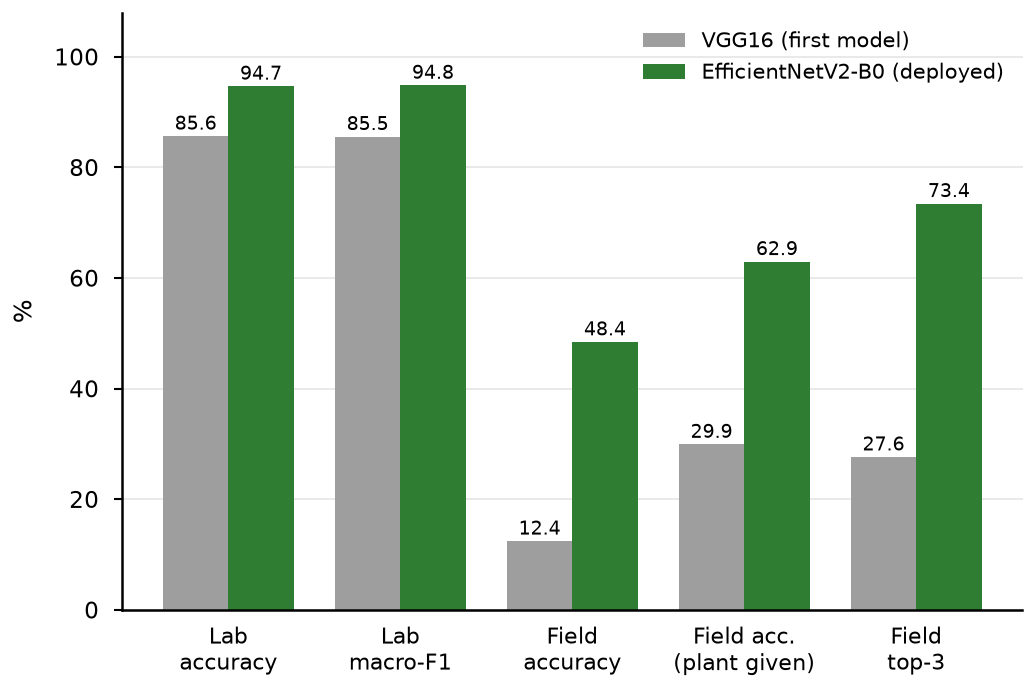
\includegraphics[width=\columnwidth]{figures/lab_vs_field.png}
\caption{Laboratory and field accuracy of the two CNNs.}
\label{fig:labfield}
\end{figure}

\subsection{Hybrid Fusion}
Table~\ref{tab:fusion} shows how the vote behaves on a tomato bacterial-spot leaf for which the CNN predicts bacterial spot at 92.5\%, under different Gemini answers. When both agree, confidence is high; an uncertain Gemini answer is outvoted by the confident CNN and the farmer is warned; conditions the CNN does not know pass through from Gemini.

\begin{table}[t]
\caption{Fusion Outcomes for a Tomato Leaf}
\label{tab:fusion}
\centering
\footnotesize
\begin{tabular}{@{}llcl@{}}
\toprule
\textbf{Gemini output} & \textbf{Final} & \textbf{Conf.} & \textbf{Label} \\
\midrule
Bacterial spot, 90\% & Bacterial spot & 91.0\% & agree \\
Early blight, 40\% & Bacterial spot & 41.0\% & cnn\_preferred \\
Early blight, 95\% & Early blight & 57.2\% & gemini\_preferred \\
Mg deficiency, 80\% & Mg deficiency & 80.0\% & gemini\_only \\
\bottomrule
\end{tabular}
\end{table}

\subsection{Yield Prediction}
A Random Forest on rainfall, pesticide use and temperature alone fails ($R^2 = -0.20$), because these values are the same for every crop in a given country and year. Table~\ref{tab:yield} shows that adding crop type, country and year fixes this, including on a temporal split that tests on later years.

\begin{table}[t]
\caption{Yield Model Feature Study}
\label{tab:yield}
\centering
\footnotesize
\setlength{\tabcolsep}{4pt}
\begin{tabular}{@{}lccc@{}}
\toprule
\textbf{Features} & \textbf{$R^2$ random} & \textbf{$R^2$ temporal} & \textbf{MAE temporal} \\
\midrule
Environment only & $-0.202$ & 0.095 & 67,359 \\
+ crop & 0.972 & 0.903 & 14,607 \\
+ crop + country & 0.974 & 0.914 & 13,835 \\
+ crop + country + year & \textbf{0.987} & \textbf{0.955} & \textbf{10,276} \\
\bottomrule
\end{tabular}
\end{table}

\section{Conclusion}
AgroTech AI combines a plant-conditioned CNN with a multimodal LLM so that any plant can be diagnosed, an offline model is kept and disagreements are visible, and it personalises advice from each farmer's records. Training on field photographs raised the CNN's field accuracy from 12.41\% to 48.43\%, and crop identity proved essential for yield prediction. Future work will add more Indian crops and field images, learn the fusion weights from data and evaluate the system with farmers.

\bibliographystyle{IEEEtran}
\bibliography{references}

\end{document}
